\documentclass[12pt]{article}
\usepackage[utf8]{inputenc}
\usepackage[T1]{fontenc}
\usepackage[french]{babel}
\usepackage{graphicx}
\usepackage{multirow}
\usepackage{wrapfig}
\usepackage{amsfonts}
\usepackage{amsmath}
\usepackage[a4paper]{geometry}
\usepackage{graphicx}
\graphicspath{ {./images/} }



\font\myfont=cmr12 at 40pt

\title{
    {\myfont Rapport De Groupe Intermédiaire} \\
    \bigskip
    Projet Tech Android
    }

    \author{Théo Dupont, Sebastian Pagès, Hugo Bergon, Elliot Renel}
    \date{28 Février 2020}

\begin{document}

\maketitle
\bigskip
\bigskip
\bigskip

\tableofcontents

\section{Structuration du Code}
    La structure globale de notre projet.\\
    \\
    \\
    \\
    Notre application MainActivity.java manipule essentiellement une classe nommée BitmapHandler, qui a la particularité de posséder deux bitmaps en son sein, ainsi que la PhotoView,
    seul place ou sera affichée la bitmap. Ainsi on manipule directement la classe BitmapHandler qui s'occupe ensuite de modifier et d'afficher la bitmap désirée en 
    les fonctions de la classe BasicFilter appellant des fonctions getPixels, setPixels.... adaptées à la structure de BitmapHandler (et non plus une bitmap simple).\\
    Ces fonctions se trouvent dans le package com.example.editionimage.imagehandling\\
    \\
    Nous avons également utilisé une nouvelle structure pour l'affichage de notre image. \\
    Nous avons donc remplacé l'ImageView par une PhotoView, qui possède comme caractéristiques les mêmes que ImageView, 
    mais auquelles on peut rajouter la faculté de scroll et de zoom de cette image.\\
    Lien: https://github.com/chrisbanes/PhotoView\\
    \\
    Kernel implémente une matrice de taille arbitraire qui sera utilisé pour n'importe quelle convolution.
    Lors d'un appel d'une fonction convolution, on peut alors créer la matrice représentant notre effet avec un Kernel.\\
    \\
    MainActivity s'occupe également de la visibilité de certains boutons comme pour le choix de la couleur à garder, ou du degré de luminosité à modifier.\\
    \\
    Cette classe manipule donc les objets produits par le fichier xml activity\_main.xml.\\
    Celui-ci est composé d'un layout qui prend la taille de l'écran, les boutons d'accès au choix de la photo, la PhotoView, et enfin, un scrollView.\\
    Ce scrollView contient toutes les fonctions de modification d'image, ainsi que d'autres scrolls, définis pour des modifications avec un choix, comme KeepColor, Colorize, et setLightlevel.
    Ces seconds scrollView sont composés d'une seekBar pour le choix de la valeur a appliquer, ainsi que d'un bouton Apply pour confirmer son choix.\\
    Toutes ces fonctions, s'il n'y a pas d'image de chargée, réalisent une erreur, d'ou notre classe ToasterNoImage, et sa fonction isToastShowed, qui teste si l'image est accessible.\\

    \bigskip

\section{Choix techniques}
    Premièrement, nous allons parler du choix de regrouper deux bitmaps en une seule dans BitmapHandler. \\
    Ceci permet de ne pas se tromper quand on appelle une fonction appellant la bitmap, et permet une bien meilleur lisibilité dans les différentes classes.\\
    \\
    La classe Kernel permet de manipuler plus simplement et plus visuellement les matrices que l'on veut appliquer. Ainsi on peut facilement appliquer une matrice dans une fonction plusieurs fois si nécessaire.
    \\
    \\
    Nous avons également utilisé des fonctions de récupération/dépot de tableaux en hsv directement, pour permettre une plus grande fluidité.
    \\
    Les fonctions de modification de contraste et de luminosité manipulent les canaux RGB car plus facile a optimiser et manipuler, que le hsv.\\
    \\



\section{Besoins fonctionnels}



    \subsection{Chargement et sauvegarde d'image}
    L'application charge correctement une image depuis la galerie, et permet également la prise de photo pour les importer dans l'application,
     avec les boutons situés en haut de l'application.\\
    L'application peut également sauvegarder, à condition d'autoriser manuellement l'application à enregistrer des photos.\\
    

    \subsection{Image et manipulation}
    L'image chargée est donc maintenant visible à l'écran, prête à être modifiée, et on peut la zoomer avec l'action des deux doigts, 
    et scroller si elle est trop grosse par rapport à la taille définie dans l'application.\\
    L'image peut également être reset avec le bouton aproprié.
    

    \subsection{Fonctions d'usage}
    Les fonctions décrites ici sont disponibles dans l'application avec les boutons dans l'ensemble de l'application, et disponibles dans la classe bitmapHandler.\\

    \begin{itemize}
        \item reset

    \subsection{Filtres}
    Les fonctions ci-dessous sont retrouvées dans la fonction BasicFilter, et testables via les boutons dans le bas de l'application.\\
    \\

    \begin{itemize}
        \item toGray():\\ 
        Transforme l'image appellante en niveau de gris.\\
        L'algorithme prend juste les niveaux de rouge, vert et bleu de l'image, en fait une moyenne pondérée avec les facteurs donnés en cours (0.3/0.59/0.11) 
        et met la moyenne comme niveau de gris dans le pixel.
        \\
        La fonction présentée dans l'application est la version renderscript, qui reprend le même principe.\\
        \\
        \item colorize(int color):\\
        Transforme l'image appellante pour que chaque pixel aie une teinte donné en paramètre.
        La méthode modifie simplement la teinte en passant les pixels en Hsv, puis en modifiant le paramètre h par celui donné en paramètre, pour repasser les pixels en rgb.\\ 
        \\
        \item keepColor(int color, int range):\\
        Transforme l'image appellante pour ne garder la couleur que de certains pixels.\\
        La methode calcule grâce aux paramètres "color" (donné dans MainActivity par une seekBar) et "range" (ici arbitraire, avec une valeur de 30 dans BitmapHandler) un intervalle de couleurs en degrés (couleur HSV) qui sont à garder. Puis dans le parcours des pixels de l'image il 
        met la saturation du pixel à 0 si sa couleur n'est pas dans l'intervalle.\\
        A noter que si l'intervalle est discontinu (couleur proche de 0 ou 360), la variable booléen "inRange" est calculée différement.\\
        \\
        \item contrastLinear():
        Transformation de contraste de manière linéaire de la bitmap appellante.\\
        Après avoir récupéré l'histogramme de l'image (histogramme de V*100 de HSV),
        on trouve les indices minimal et maximal non nuls dans l'histogramme, afin d'appliquer la formule Range*(Valeur-Min)/(Max-Min) où Valeur est 
        la valeur du pixel en cours (V*100 pour Color) et Range est la taille des valeurs possible -1. Pour l'histogramme la valeur V utilisée pour l'indice est multiplié par 100 pour pouvoir avoir des indices de tableau 
        déscents, puis redivisé par 100 une fois récupéré.\\
        \\
        \item contrastEqual():
        Transformation de contraste par égalisation d'histogramme du BitmapHandler appellant.\\
        Après avoir récupéré l'histogramme de l'image (de la même manière que le contraste linéaire) et calculé l'histogramme cumulé C[],
        on calcule pour chaque pixel la valeur C[Value]*Range/Size où Value et Range ont le même rôle que dans le contraste linéaire 
        et Size est le nombre de pixels de l'image. La valeur de V pour l'histogramme est aussi multiplié par 100 
        pour les mêmes raison que ci-dessus, puis de-même redivisé par 100.\\
        En RS: La fonction d'égalisation d'histogramme renderscript convertit l'image au format YUV qui sépare le luma des couleurs (chrominance) pour ne traiter qu'un seul canal.\\
        \\
        \item modifLight(double alpha):   
        Modification de la luminosité de l'image appellante.
        La fonction ajoute/réduit jusqu'a une valeur de 80 a chaque canal rouge, vert et bleu simultanément pour faire varier la luminosité de chaque pixel.\\
        \\
        \item modifLight(double alpha):   
        Modification du contraste de l'image appellante.
        Cette fonction utilise la valeur donnée pour augmenter ou réduire les canaux du pixel en conséquence, par rapport à ses canaux de base. Ainsi les canaux élevés seront augmentés alors que ceux qui sont faibles seront plus proches de 0.\\
        \\
    \end{itemize}

    \subsection{Convolutions}
        Toutes les fonctions de convolution présentées ici sont appliquées de la même manière.
        On crée un Kernel avec les données que l'on veut rentrer (la matrice du flou gaussien par exemple.)
        On donne ensuite ce noyau a applyMask qui donnera les nouvelles valeurs après passage de la matrice sur l'image.
        Puis on actualise notre bitmap courante.

    \begin{itemize}
        
        \item GaussianBlur():
        Gaussian est une application de flou gaussien avec une matrice de Gauss de dimension 5*5 comme ci-dessous.
            \begin{equation}
                \begin{pmatrix}
                    1 & 4 & 6 & 4& 1\\
                    4 & 16 & 24 & 16 & 4\\
                    6 & 24 & 36 & 24 & 6\\
                    4 & 16 & 24 & 16 & 4\\
                    1 & 4 & 6 & 4 & 1\\
                \end{pmatrix}
            \end{equation} 
        \\
        \item simpleEdgeDetection()(Laplace): 
        simpleEdgeDetection est une application de la détection de bordure de Laplace avec une distribution gaussienne, Laplace étant utilisé pour la détection de bords.
        \begin{equation}
            \begin{pmatrix}
                0 &  0 & -1 &  0 &  0\\
                0 & -1 & -2 & -1 &  0\\
                -1 & -2 & 16 & -2 & -1\\
                0 & -1 & -2 & -1 &  0\\
                0 &  0 & -1 &  0 &  0
            \end{pmatrix}
        \end{equation} 
        \\
        \item Sobel():
        Sobel est un autre moyen de réaliser la détection des bords.
        Il utilise ces deux matrices 3x3 ci-dessous, avec la première qui réalisera la détection de bord verticaux et la deuxième ceux horizontaux
        (cela simule l'effet d'une grosse matrice d'une manière plus efficace):
        \begin{equation}
            \begin{pmatrix}
                1 &  0 & -1 \\
                2 & 0 & -2 \\
                1 & 0 & -1 \\
            \end{pmatrix}
        \end{equation} 
        \begin{equation}
            \begin{pmatrix}
                1 &  2 & 1 \\
                0 & 0 & 0 \\
                -1 & -2 & -1 \\
            \end{pmatrix}
        \end{equation} 
        
    
    \end{itemize}

\subsection{Nouveaux Effets}

Pour montrer l'utilité de nos fonctions précédentes nous avons créé des effets plus complexes qui les utilisent .
\begin{itemize}
    \item crayonEffect():
    A partir d'une image, ce filtre donne un effet crayon.

    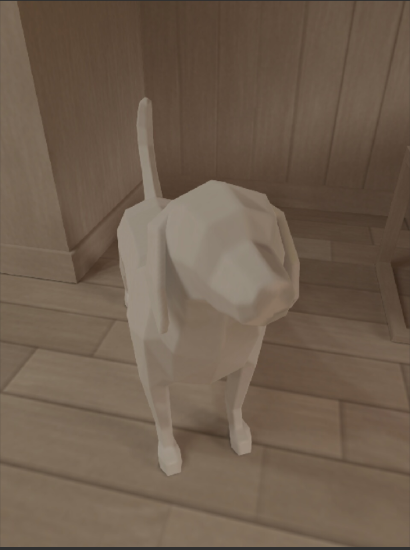
\includegraphics{dog_original}

    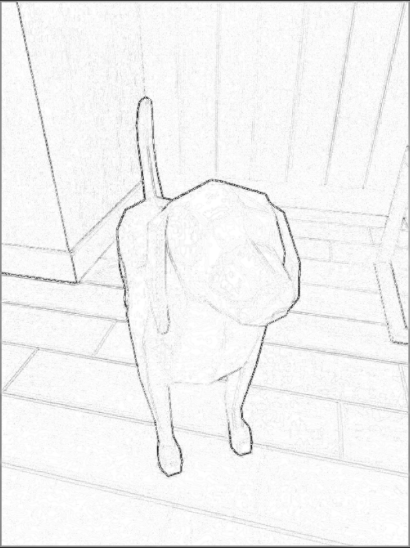
\includegraphics{dog_crayon}

    \item cartoonEffect():
    Cet effet donne un effet bande dessiné à une image.

    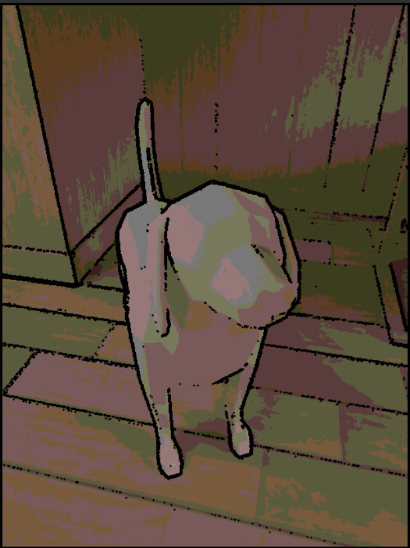
\includegraphics{dog_cartoon}

\end{itemize}

\subsection{Pile d'effets}

\begin{itemize}
Nous avons ajouté la possiblité de défaire des modifcations en enregistrant les effets successifs afin de pouvoir récréer un état anterieur de l'image.

Ces états sont empilés au fur et a mesure de leur utilisation dans l'application, et sont dépilé après l'utilisation d'un des effets suivants.\\

\item Save:
Le bouton save utilise cette pile d'effets avec une troisième bitmap, bit_final, qui est de taille d’origine par rapport à l’image effectuée, et utilise une pile d’effets pour les appliquer a cette bitmap, puis l’enregistrer et retrourner le ficher crée.
\\

\item Undo:
Le bouton undo utilise également cette pile en récupérant la dernière action et en l'annulant. Il retire également l'effet de la pile.
\\

\item Reset:
    Le bouton reset réinitialise l’image affichée a l’image importée au départ.
    On utilise pour cela deux bitmaps différentes, une courante, affichée sur l’application, et une originale qui sera utilisée pour remettre l’image courante comme celle de base.\\
    \\

\end{itemize}

\section{Problèmes connus}

\begin{itemize}
    \item Les images sont sauvegardées sur le téléphone dans un dossier dédié dans le dossier de base des photos, mais ce dossier n'est pas visible depuis la gallerie.\\
    \item Les fonctions de conversion hsv renderscript ne fonctionnent pas (l'image n'est pas celle attendue). Tous les fichiers renderscript sont dans le dossier ./projet/src/rs/ mais seuls gray.rs et histEq.rs sont appellés.\\
\end{itemize}




\section{profilage}
 \bigskip
    Le profilage  a été réalisé sur trois dimensions d’images : une image « petite » 259*194 pixels,  une image « camera » provenant de l’appareil photo du téléphone 960*1280 pixels et l’image « centrale » qui est l’image redimensionnée au centre de l’application servant de prévisualisation des effets avant leurs sauvegarde.\\
    Toutes les valeurs et images sont issues du profilage d’un émulateur d’un appareil PIXEL 2 XL, sous l’API 29.\\

    Les valeurs sont issues de moyennes sur une dizaines de lancés. \\
    Le temps que prend un effet est calculé a partir de la première trace d’activité du processeur après le déclenchement du bouton correspondant a l’effet et se termine lorsque l’activité du processeur se stabilise à zéro.\\
    La mémoire utilisées est calculé en faisant la somme de chaque  croissance de la mémoire utilisée soustrait par l’utilisation de mémoire avant cette croissance. Le garbage collector s’enclenchant souvent au début d’un effet, ou lors des effets plus long à calculé, plusieurs fois de manières périodique (voir l’image du profileur de linear contrast). Le garbage collector (GB) influence l’utilisation de la mémoire mais aussi celle du processeur, deplus, le profileur affecte aussi grandement le temps que met un effet a se terminer. Le profilage ne montre pas réellement l’utilisation de la mémoire par un effet, mais l’utilisation dans un contexte. Ainsi on peut comparer, sur un contexte en tout point similaire sauf les dimensions de l’images sur laquelle est appliqué l’effet, les utilisations des ressources de l’appareil.\\
   
 Tout d’abord nous allons faire le profilage des effets indépendamment des uns et des autres sur l’image « centrale ». \\
    Ensuite nous ferons un profilage comparant l’utilisation de ressources sur l’image « petite » et de l’image provenant de l’appareil photo.\\

 \bigskip
 \bigskip
 \bigskip
 \bigskip
 \bigskip
 \bigskip
 \bigskip
 \bigskip

 \bigskip




   \subsection{Profilage des effets individuels} 

 \bigskip


    Togray : mémoire moyenne utilisées 2,7mB, temps moyen 0,684s.\\




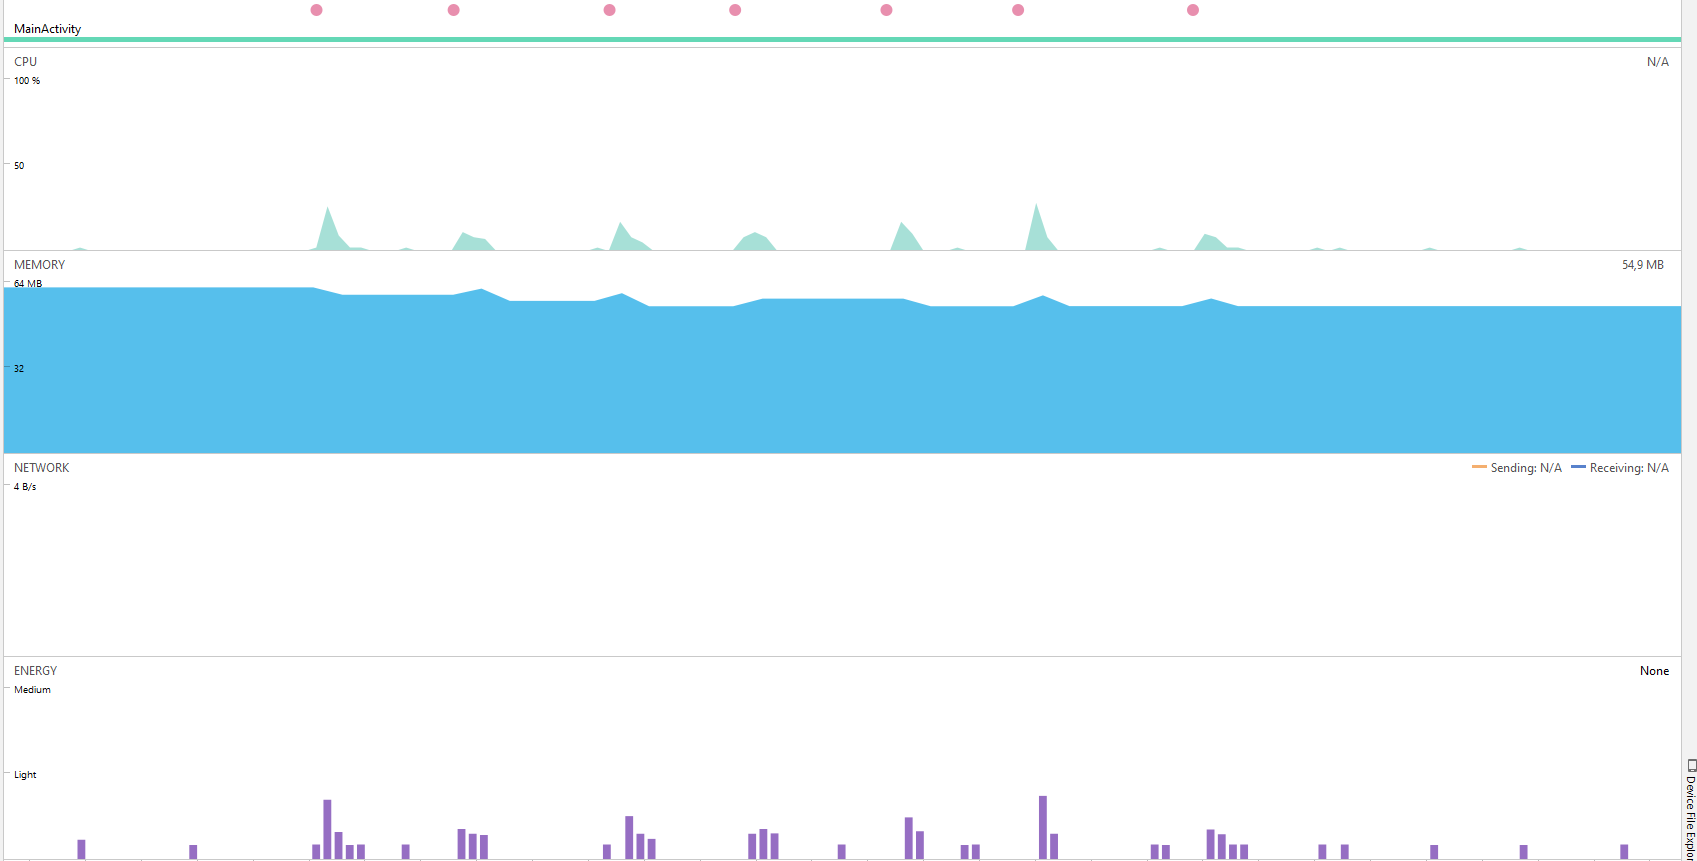
\includegraphics[width=\textwidth]{1-togray}\\


    Remarque :
    Les effets togray, keep color et shift ont des allures très similaires, une seule image de profileur est donc présentée.\\

 \bigskip




    Colorize : mémoire  mémoire moyenne utilisée 11,3mB, temps moyen 0,537s.\\

    Remarque :
    Sur plusieurs lancés de colorize, le GB se lance deux fois d’affilés lors du même lancé. Ainsi en prenant en compte ces lancés fortement influencé par le GB l’utilisation moyen de la mémoire serait  de 7,8mB.\\

 \bigskip



    Keep Color : mémoire moyenne utilisée 10,2mB, temps moyen 0,528s.\\

 \bigskip




    Shift : mémoire moyenne utilisée 9,5mB, temps moyen 0,494s.\\




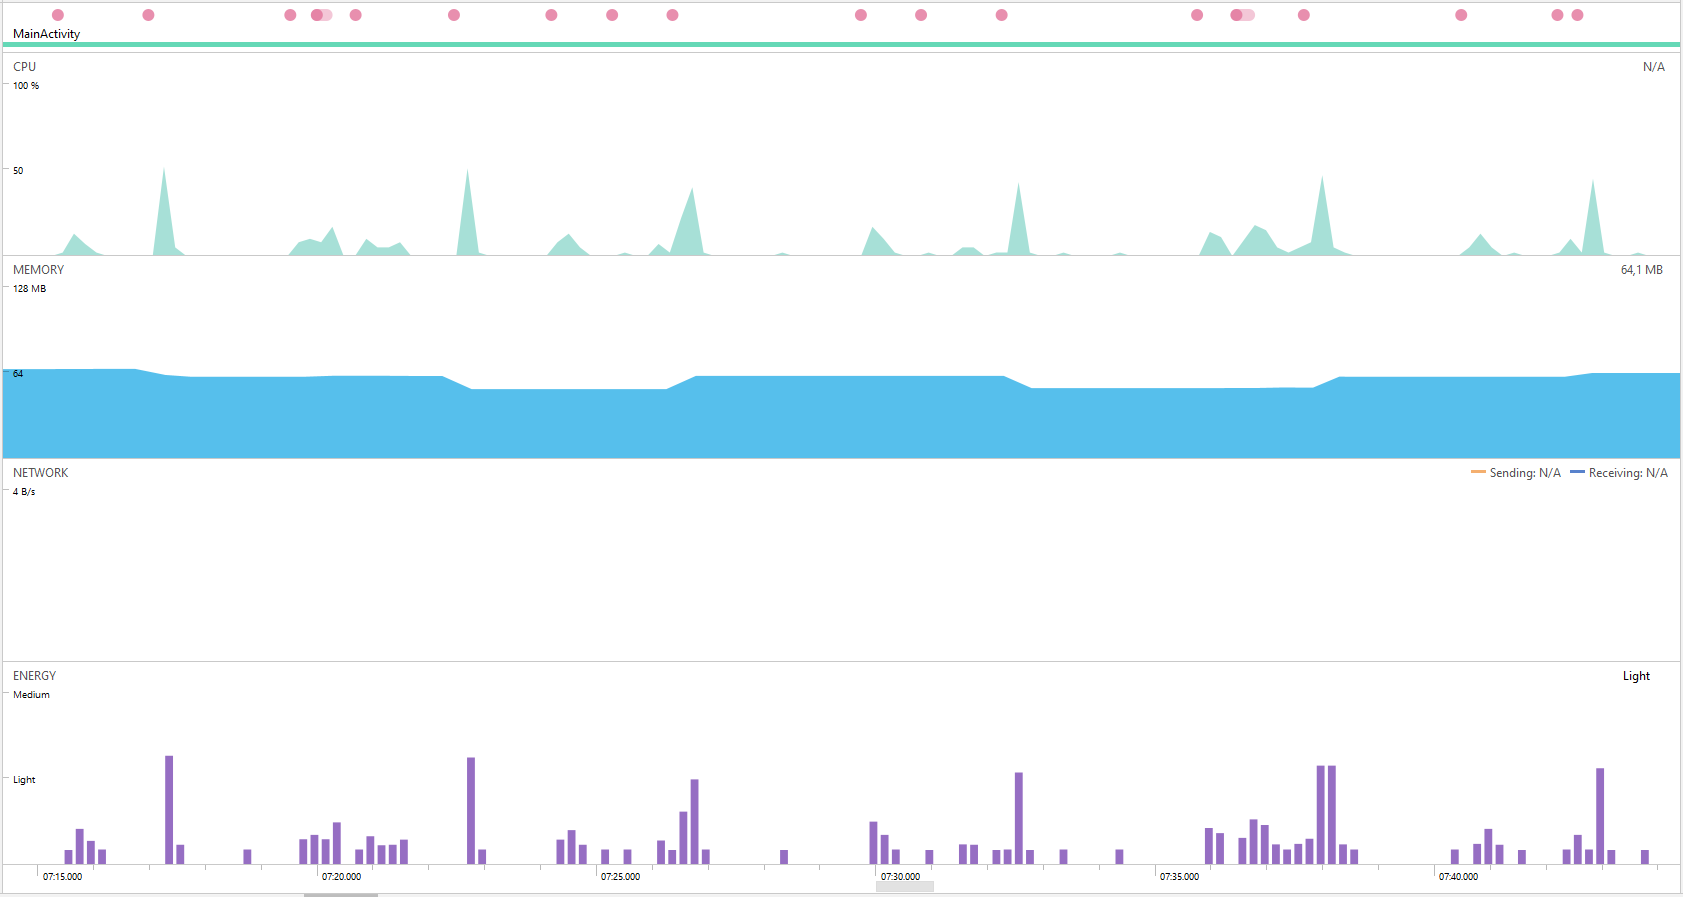
\includegraphics[width=\textwidth]{1-shift}

 \bigskip



Linear contrast : mémoire moyenne utilisée 39mB, temps moyen 40,4s.\\

 \bigskip
Première partie :\\
 \bigskip

    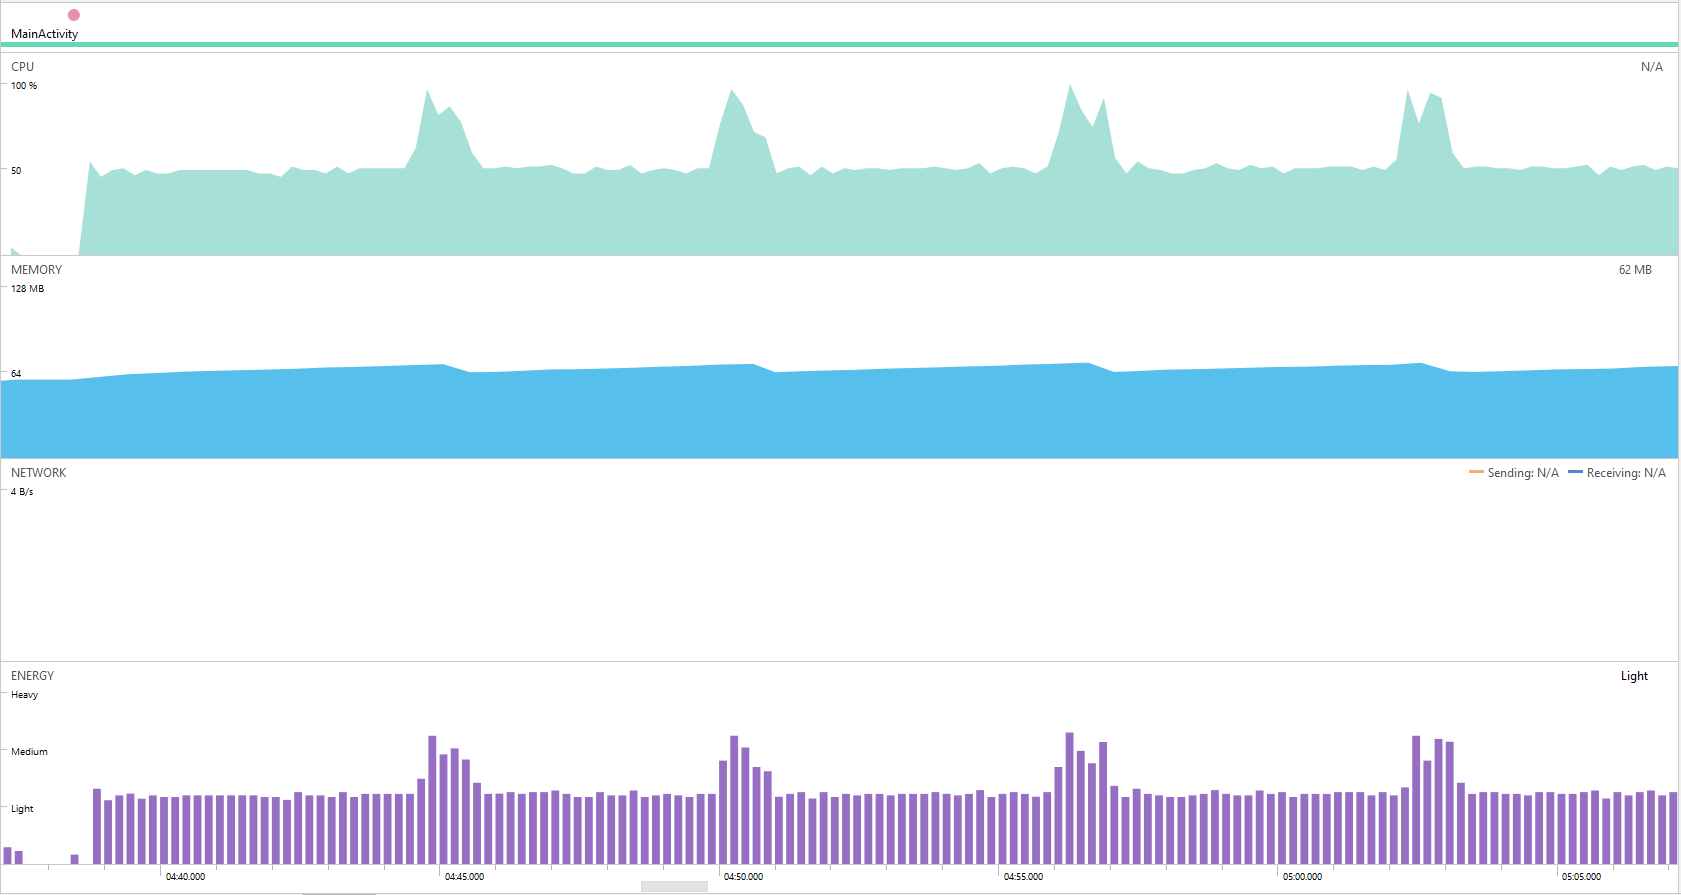
\includegraphics[width=\textwidth]{linelong1}
 \bigskip
 \bigskip
 \bigskip
 \bigskip

 \bigskip
Seconde partie :\\
 \bigskip
    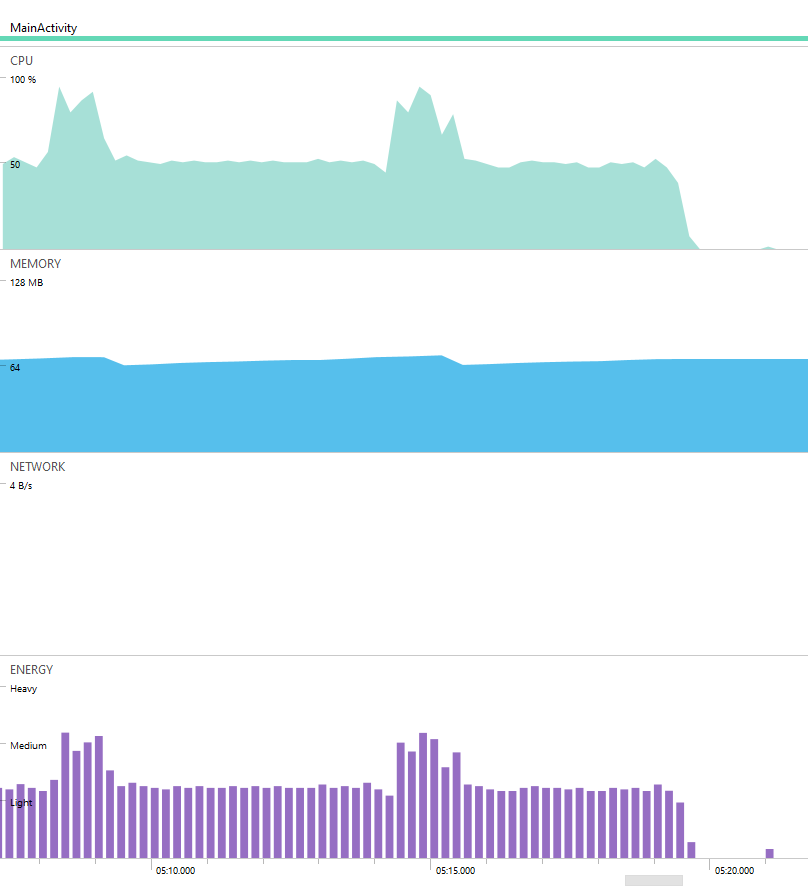
\includegraphics[width=\textwidth, height = 7cm]{linelong2}

    Remarque : 
    Les effets utilisant des histogrammes (sauf equalizer contrast) ainsi que les fonctions utilisant la convolution ont une allure similaire a Linear contrast, très longue et des utilisations de la mémoires en « dents de scie » entrecoupés par le GB qui arrive souvent après avoir atteint une certaine valeur mémoire utilisée.\\
    Ici le GB arrivait sur 5 des 6 dents de scie, chacune culminant à 5,5mB de plus que leurs bases.\\

 

    Equalizer contrast : mémoire moyenne utilisée 2,7mB, temps moyen 0,760s.\\





    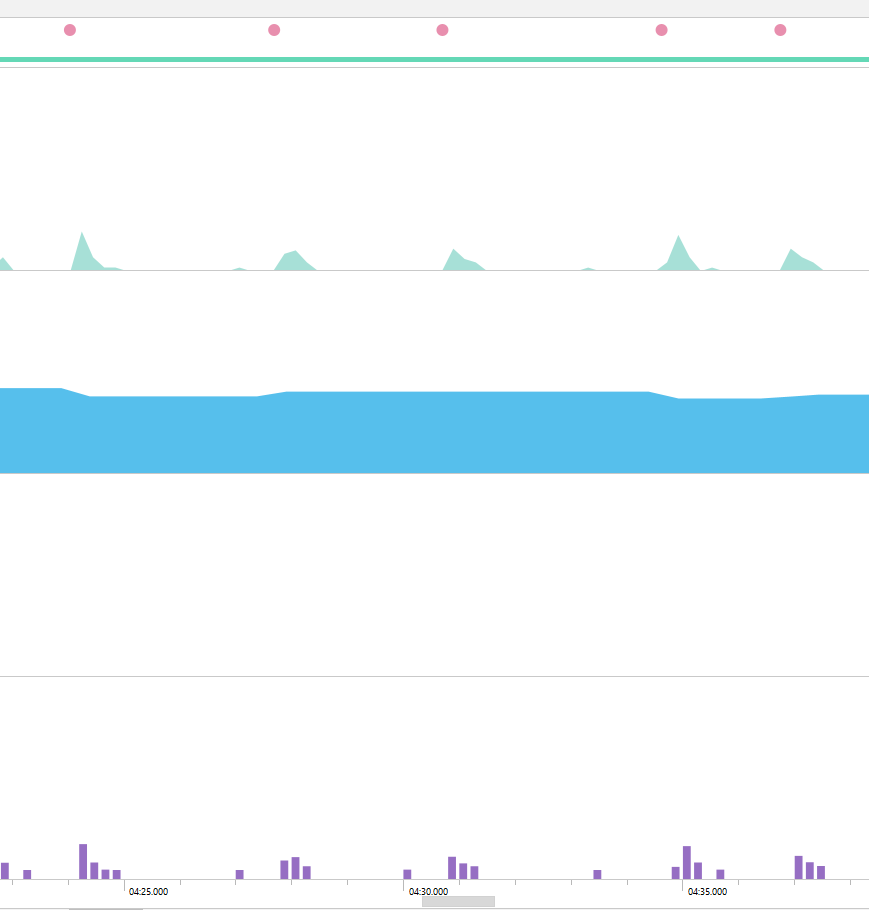
\includegraphics[width=\textwidth, height = 7cm]{egalisateur}



    Remarque :
    Comme dit précédemment elle diffère des autres fonctions utilisant des histogrammes, cela est peut-être du au fait que c'est la seule à utiliser un histogramme cumulé.\\

 \bigskip




    Modify contrast : mémoire moyenne utilisée 1,4mB, temps moyen 0,576s.\\



    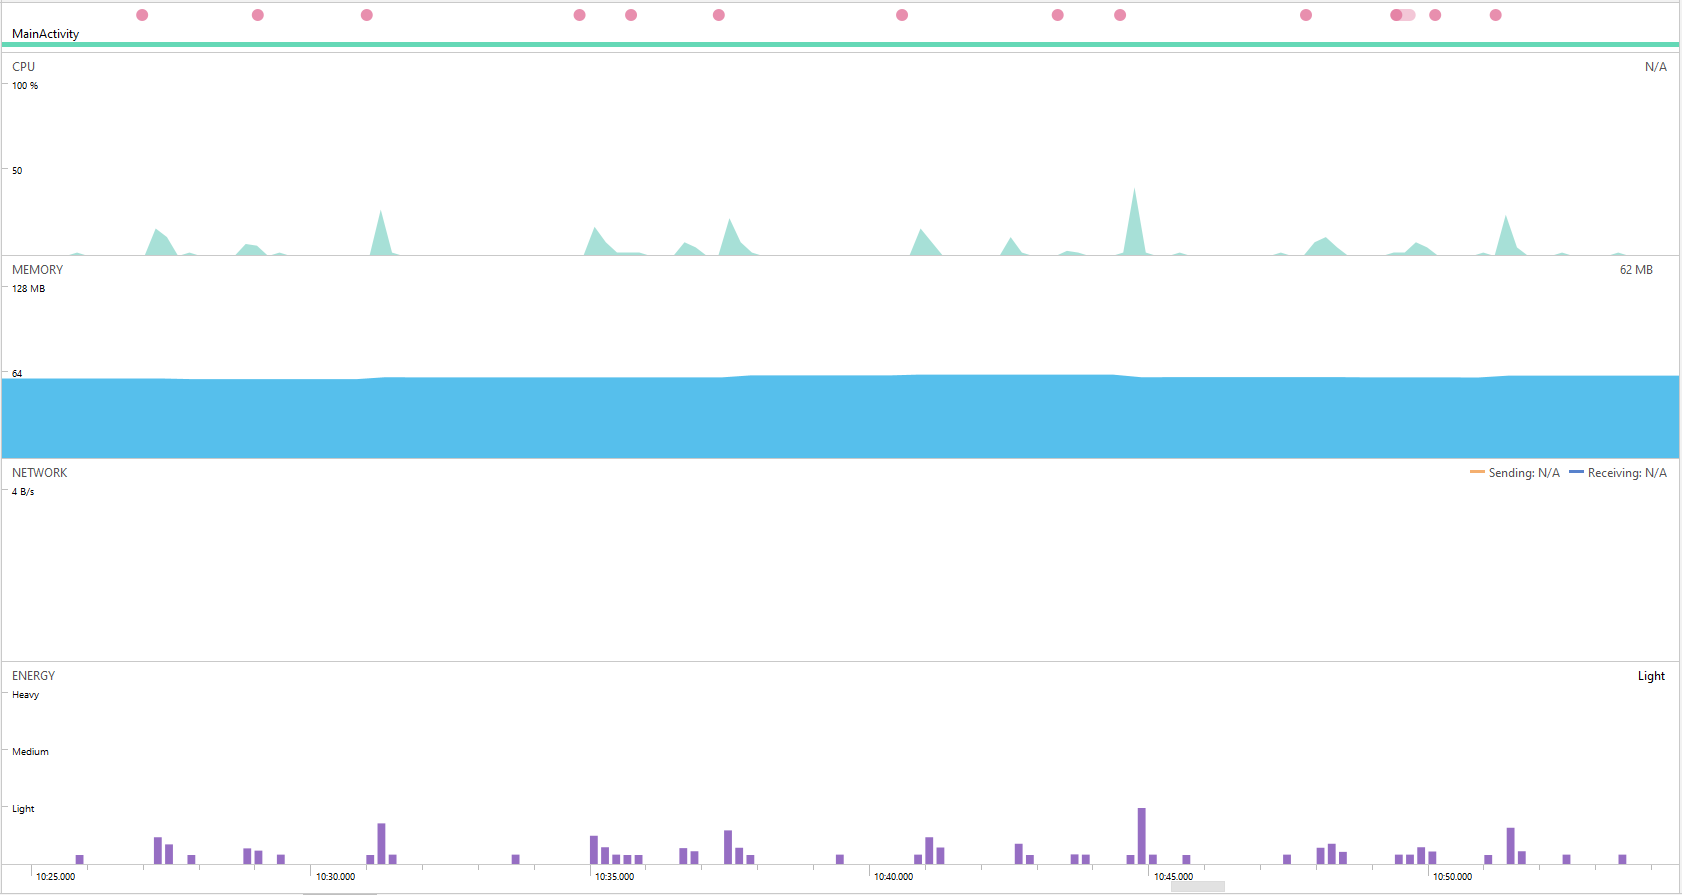
\includegraphics[width=\textwidth]{modifycontrast}

 \bigskip





    Modify lightlevel : mémoire moyenne utilisée 1,4mB, temps moyen 0,512s.\\



    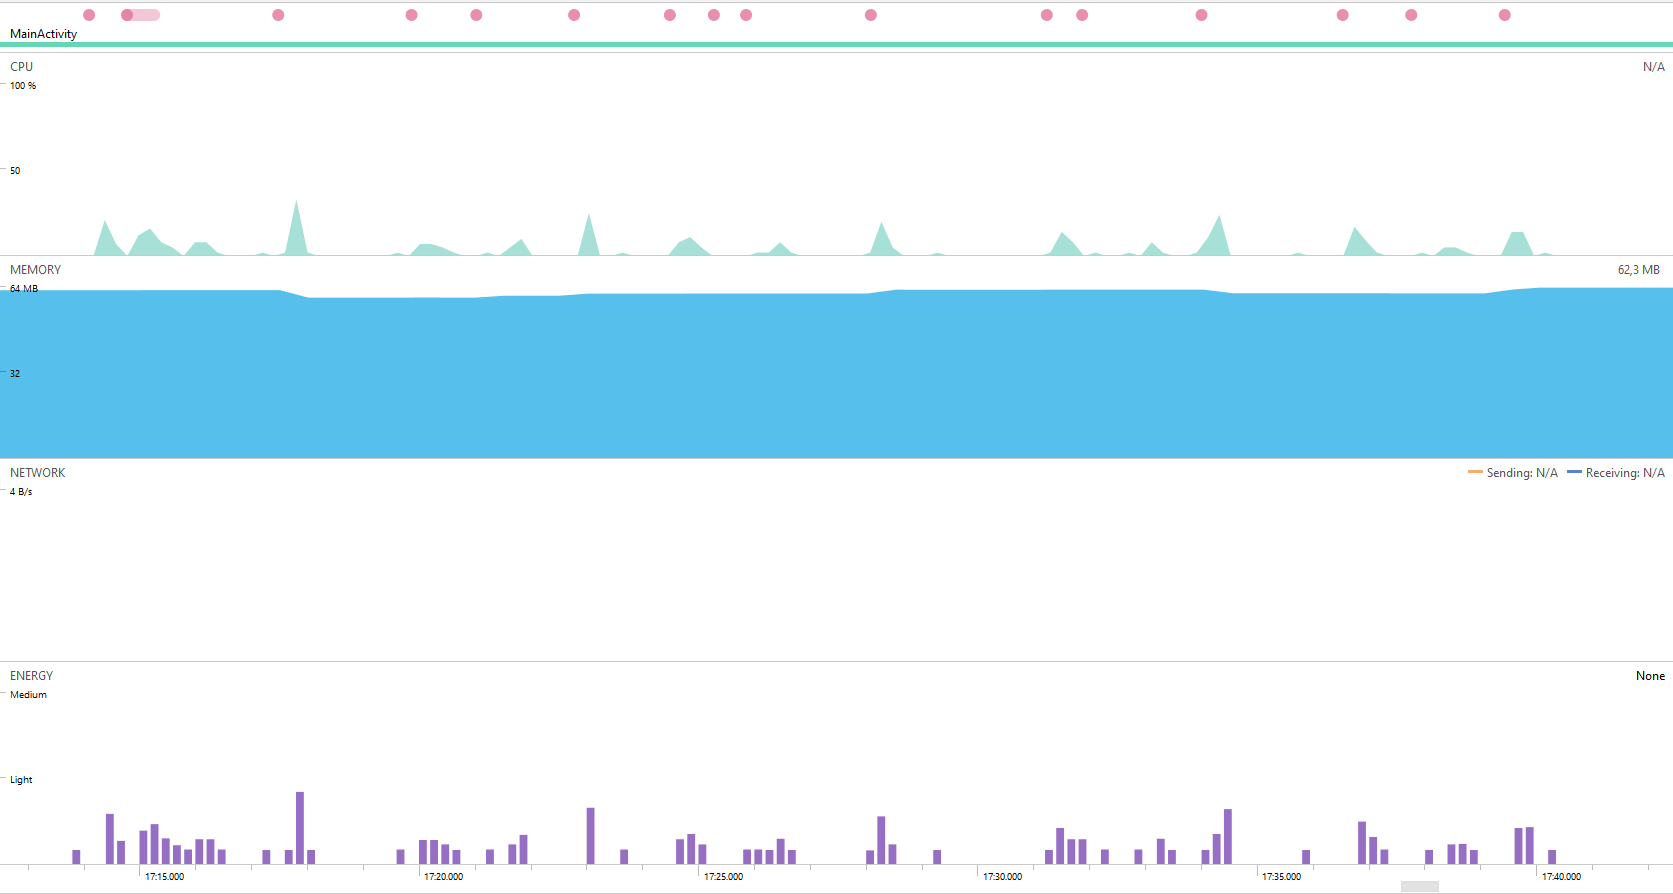
\includegraphics[width=\textwidth]{modifylight}

 \bigskip






    Gaussian blur  : mémoire moyenne utilisée 42mB, temps moyen 40,674s.\\

 \bigskip




    Laplacian edge detection : mémoire moyenne utilisée 44,8mB, temps moyen 39,949s.\\

 \bigskip




    Sobel edge detection : mémoire moyenne utilisée 39,6mB, temps moyen 40,637s.\\

 \bigskip




    Crayon effect : mémoire moyenne utilisée 48,5mB, temps moyen 40,312s.\\

 \bigskip




    Cartoon effect : mémoire moyenne utilisée 43,4mB, temps moyen 39,353s.\\

 \bigskip





     \subsection{profilage comparatif } 
 \bigskip



    Les comparaisons se basent sur 2 protocoles : le premier est l’appel à l’effet linear contrast  puis le bouton save. L’autre protocole est l’appel consécutif des effets togray, colorize, keep color et shift puis save. \\


    Protocole 1 : linear contrast.\\

    Image « camera » : mémoire moyenne utilisée 168mB, temps moyen 1min39,114s.\\

    Remarque :
    L’allure est similaire a celle de linear contrast mais est beaucoup plus longue. \\


    Image «petite» : mémoire moyenne utilisée 8mB, temps moyen 6,2s.\\

    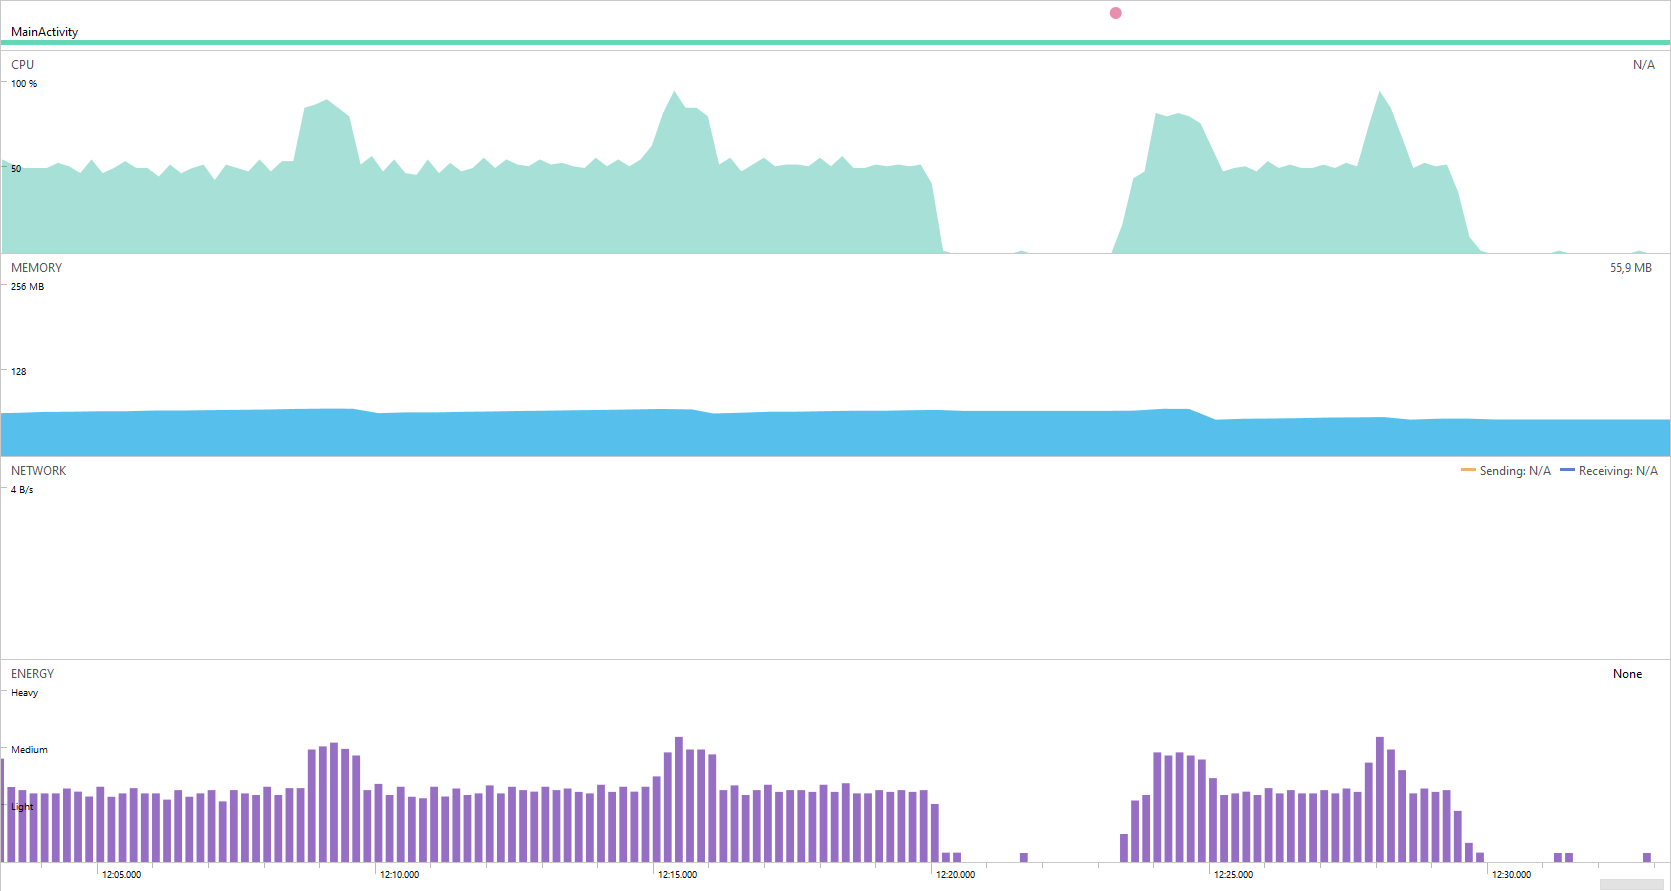
\includegraphics[width=\textwidth]{petite-linear}
 \bigskip



    Remarque :
    On voit une petite partie, à droite, de l’effet linear contrast sur l’image « centrale » et à gauche le même effet lorsqu il est vraiment appliqué sur l’image plus petite.\\


    Protocole 2 : togray + colorize + keep color + shift.\\

    Image « camera » : mémoire moyenne utilisée 30mB, temps moyen 1,590s.\\


    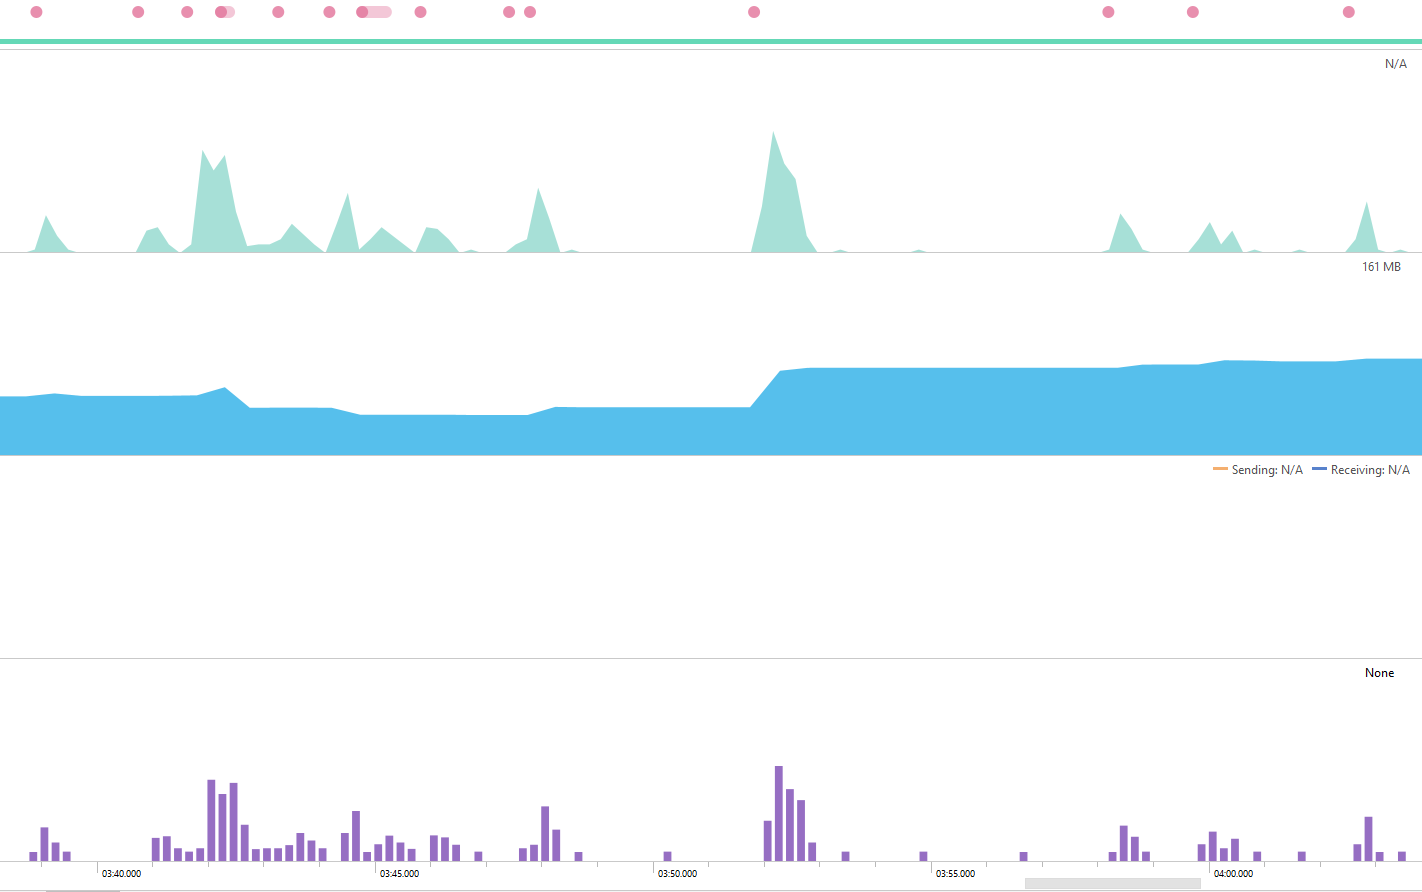
\includegraphics[width=\textwidth]{camera-serie}
 \bigskip



    Remarque :
    On voit d’abord la suite des effets sur la partie de gauche, au centre la première sauvegarde (les moyennes ont été calculées sur la première sauvegarde puis le protocole est relancé) et a droite d’autres appel du bouton save. On remarque que la première save est plus longue et plus gourmande  que les suivantes. Ce phénomène arrivait aussi sur d’autres effets mais plus rarement et beaucoup moins signifiant.\\


    Image «petite» : mémoire moyenne utilisée 4,5mB, temps moyen 0,586s.\\


    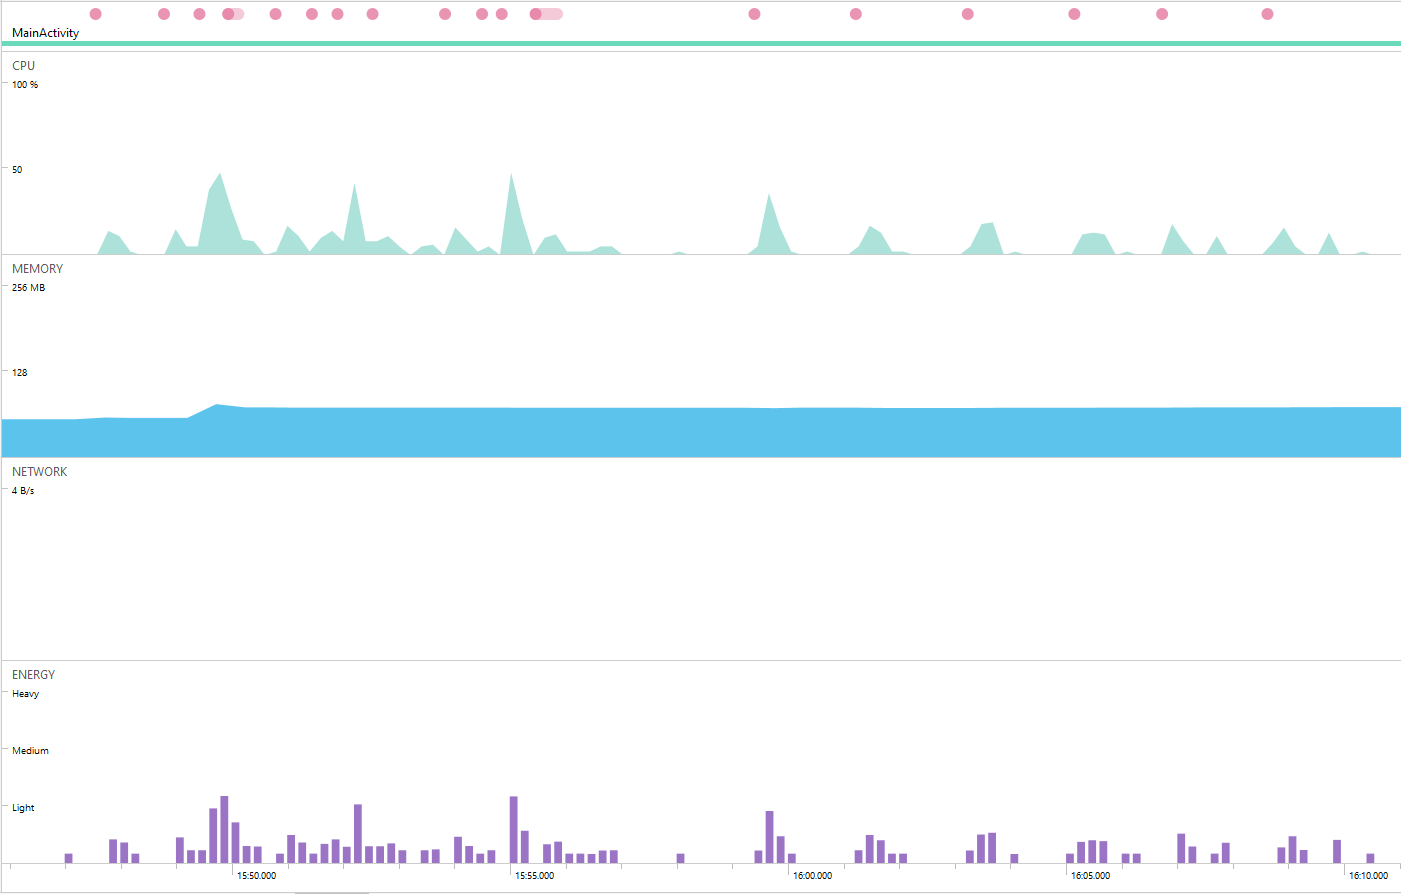
\includegraphics[width=\textwidth]{petite-serie}
 \bigskip


    Remarque :
    On voit à gauche la suite d’effet du protocole 2 et à droite une suite de save. On remarque à nouveau que le premier save est plus long que les autres.\\






\end{document}